\chapter{Data Structures}

This appendix summarizes, for reference purposes, all descriptor and
block layouts in Icon.

\section{A.1 Descriptors}

Descriptors consist of two words (normally C ints): a d-word and a
v-word. The d-word contains flags in its most significant bits and
small integers in its least significant bits. The v-word contains a
value or a pointer. The flags are


\ \ n\ \ nonqualifier\newline
\ \ p\ \ v-word contains a pointer\newline
\ \ v\ \ variable\newline
\ \ t\ \ trapped variable

\subsection{A.1.1 Values}

There are three significantly different descriptor layouts for
values. A qualifier for a string is distinguished from other
descriptors by the lack of an n flag in its d-word, which contains
only the length of the string. For example, a qualifier for the string
{\textquotedbl}hello{\textquotedbl} is


\bigskip


\bigskip


\bigskip


\bigskip


The null value and integers have type codes in their d-words and are
self-contained. Examples are:


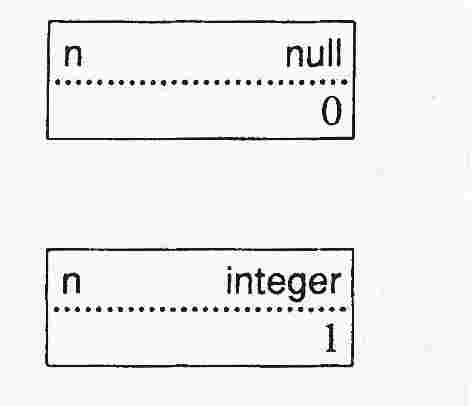
\includegraphics[width=1.602in,height=1.3547in]{ib-img/ib-img111.jpg} 


For all other data types, a descriptor contains a type code in its
d-word and a pointer to a block of data in its v-word. A record is
typical:


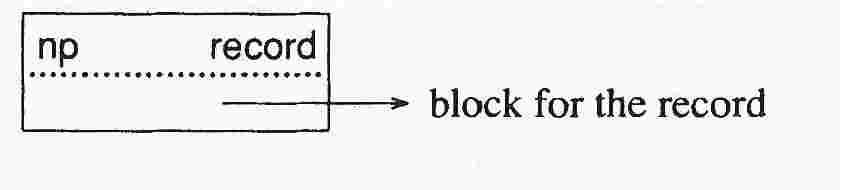
\includegraphics[width=2.8846in,height=0.6335in]{ib-img/ib-img112.jpg} 

\subsection[A.1.2 Variables]{A.1.2 Variables}

There are two formats for variable descriptors. The v-word of an
ordinary variable points to the descriptor for the corresponding
value:


\bigskip


If the variable points to a descriptor in a block, the offset is the
number of \textit{words} from the top of the block to the value
descriptor. If the variable points to a descriptor that corresponds to
an identifier, the offset is zero.


The descriptor for a trapped variable contains a type code for the
kind of trapped variable in its d-word and a pointer to the block for
the trapped variable in its v-word. The trapped variable for \&subject
is typical:


\ \  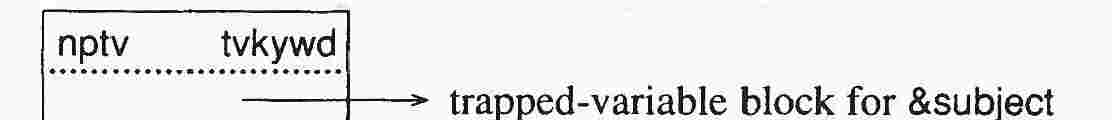
\includegraphics[width=3.7402in,height=0.4008in]{ib-img/ib-img113.jpg} 

\section[A.2 Blocks]{A.2 Blocks}

With the exception of the null value, integers, and strings, the data
for Icon values is kept in blocks. The first word of every block is a
title that contains the type code for the corresponding data type. For
blocks that vary in size for a particular type, the next word is the
size of the block in bytes. The remaining words depend on the block
type, except that all non-descriptor data precedes all descriptor
data. With the exception of the long integer block, the diagrams that
follow correspond to blocks for computers with 32-bit words.

\subsection[A.2.1 Long Integers]{A.2.1 Long Integers}

On computers with 16-bit words, integers that are too large to fit in
the d-word of a descriptor are stored in blocks.  For example, the
block for the integer 80,000 is


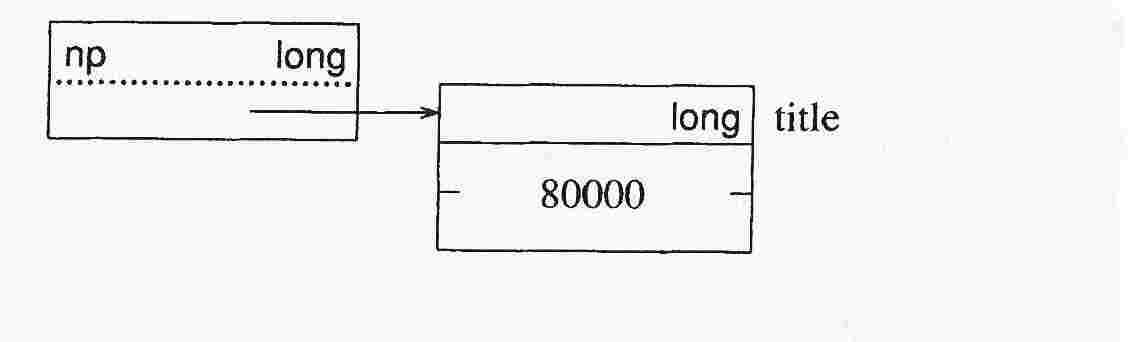
\includegraphics[width=3.848in,height=1.1425in]{ib-img/ib-img114.jpg} 

\subsection[A.2.2 Real Numbers]{A.2.2 Real Numbers}

Real numbers are represented by C doubles. For example, on computers
with 32-bit words, the real number 1.0 is represented by


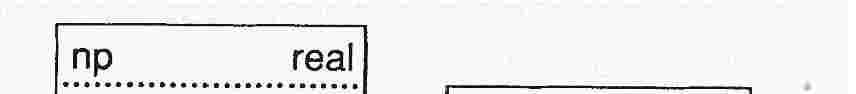
\includegraphics[width=2.8846in,height=0.3134in]{ib-img/ib-img115.jpg} 

\subsection{A.2.3 Csets}

The block for a cset contains the usual type code, followed by a word
that contains the number of characters in the cset. Words totaling 256
bits follow, with a one in a bit position indicating that the
corresponding character is in the cset, and a zero indicating that it
is not. For example, \&ascii is

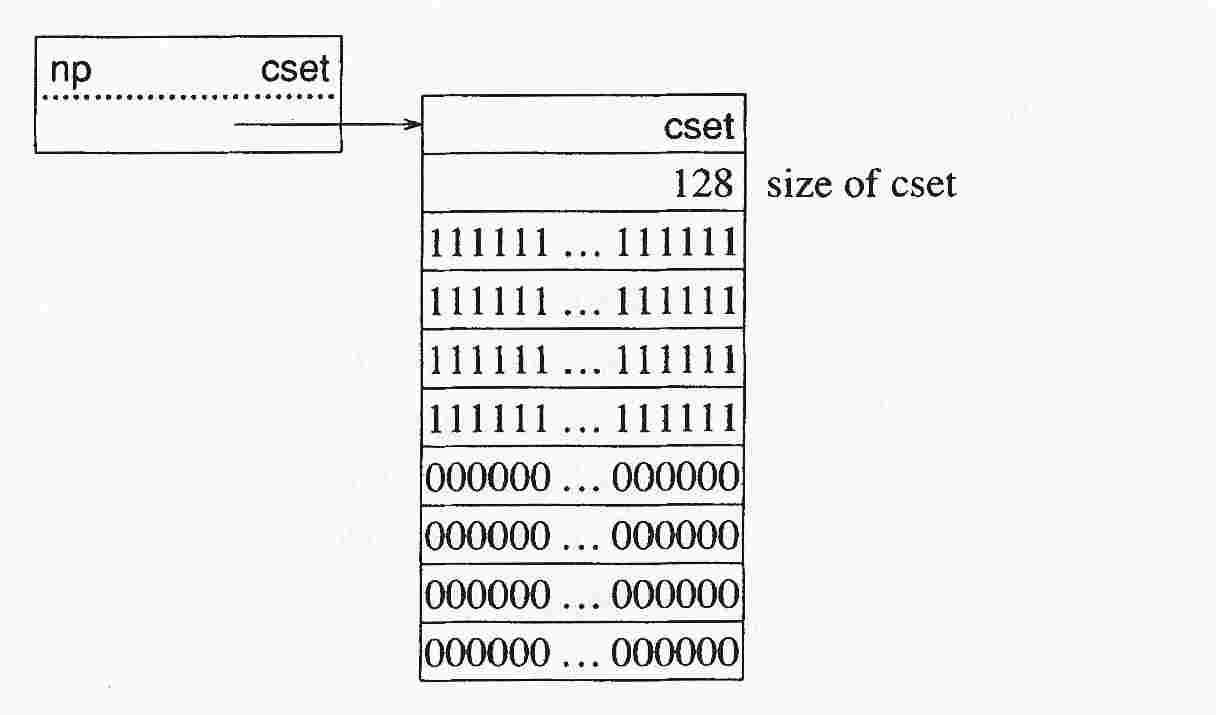
\includegraphics[width=4.0602in,height=2.3874in]{ib-img/ib-img116.jpg} 

\subsection{A.2.4 Lists}

A list consists of a list-header block that points to a doubly-linked
list of list-element blocks, in which the list elements are stored in
circular queues. See Chapter 6 for details. An example is the list

{\ttfamily\mdseries
\ \ [1,2,3]}

\noindent which is represented as


\ \  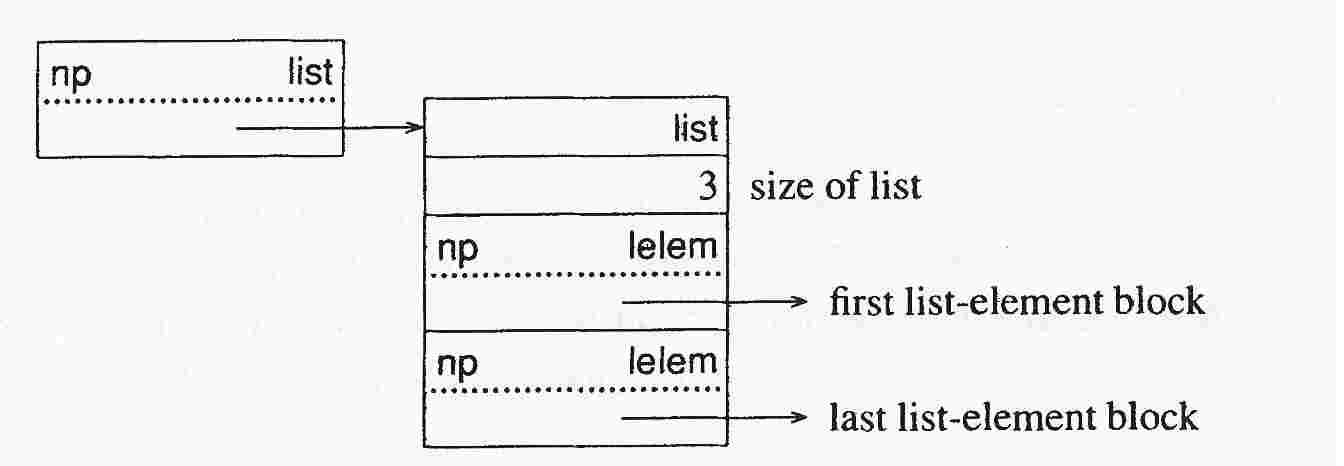
\includegraphics[width=4.489in,height=1.5563in]{ib-img/ib-img117.jpg} 


Here there is only one list-element block:


\ \  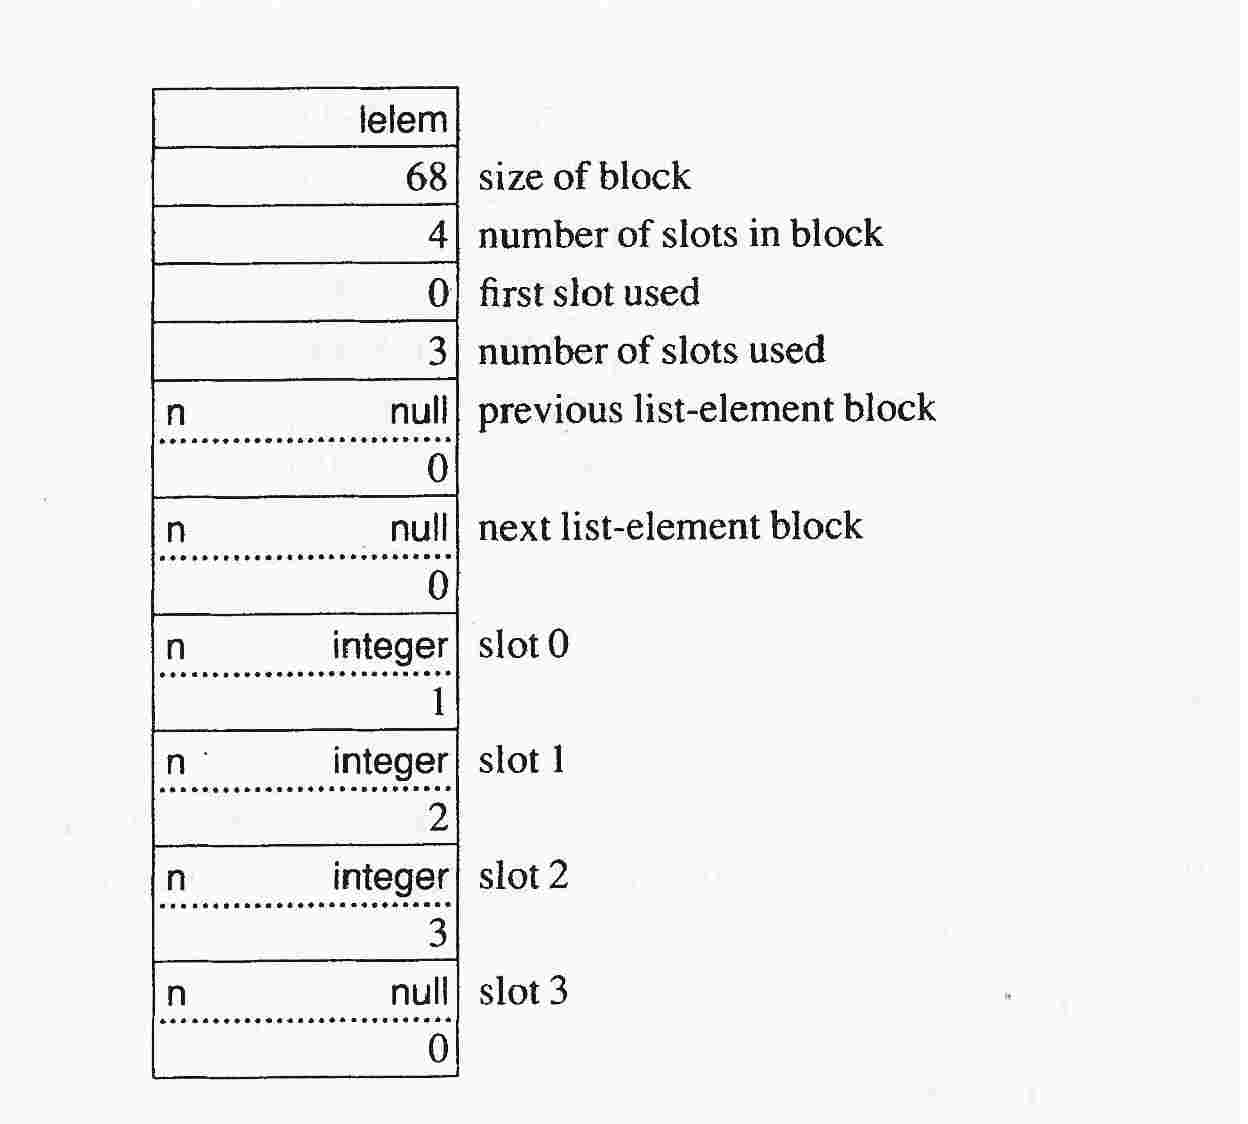
\includegraphics[width=4.1681in,height=3.7543in]{ib-img/ib-img118.jpg} 

\subsection{A.2.5 Sets}

A set consists of a set-header block that contains slots for linked
lists of set-element blocks. See Sec. 7.1 for details. An example is
given by

{\ttfamily\mdseries
\ \ set([1, 2, 3, 4])}

\noindent which is represented as


\ \  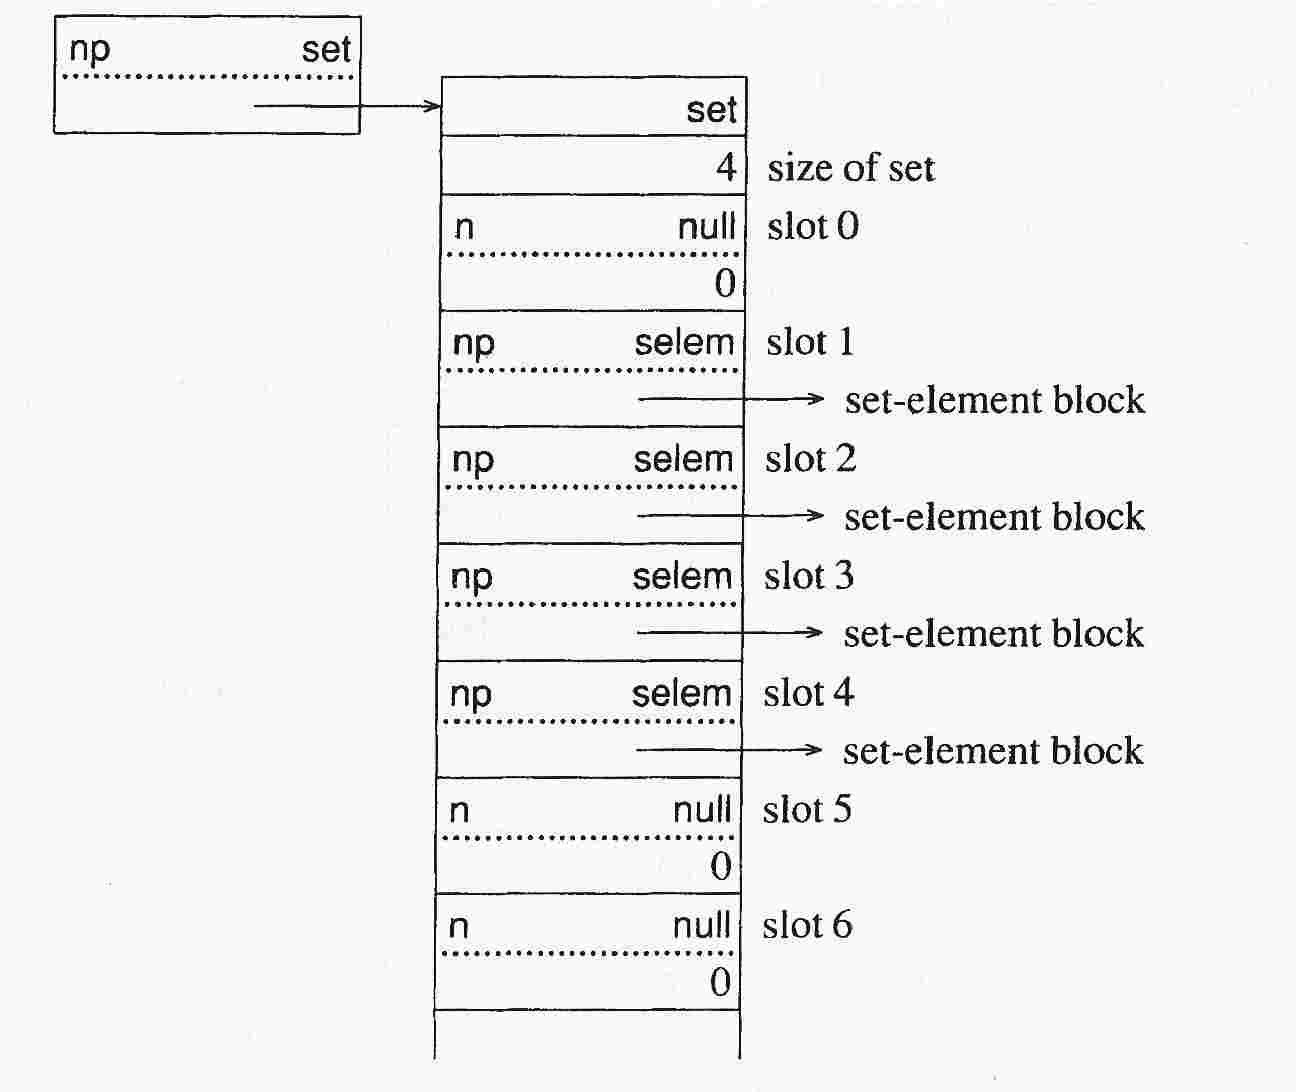
\includegraphics[width=4.3811in,height=3.6465in]{ib-img/ib-img119.jpg} 


The set-element block for the member 3 is


\ \  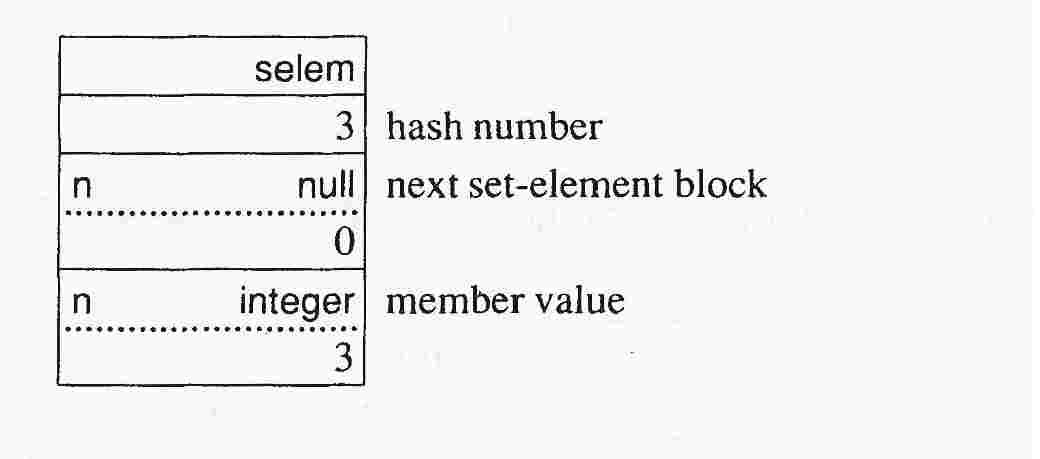
\includegraphics[width=3.5272in,height=1.5319in]{ib-img/ib-img120.jpg} 

\subsection{A.2.6 Tables}

A table is similar to a set, except that a table-header block contains
the default assigned value as well as slots for linked lists of
table-element blocks. See Sec. 7.2 for details. An example is given by

{\ttfamily\mdseries
\ \ t := table()}

{\ttfamily\mdseries
\ \ every t[1 {\textbar} 4 {\textbar} 7] := 1}


The table t is represented as


\ \  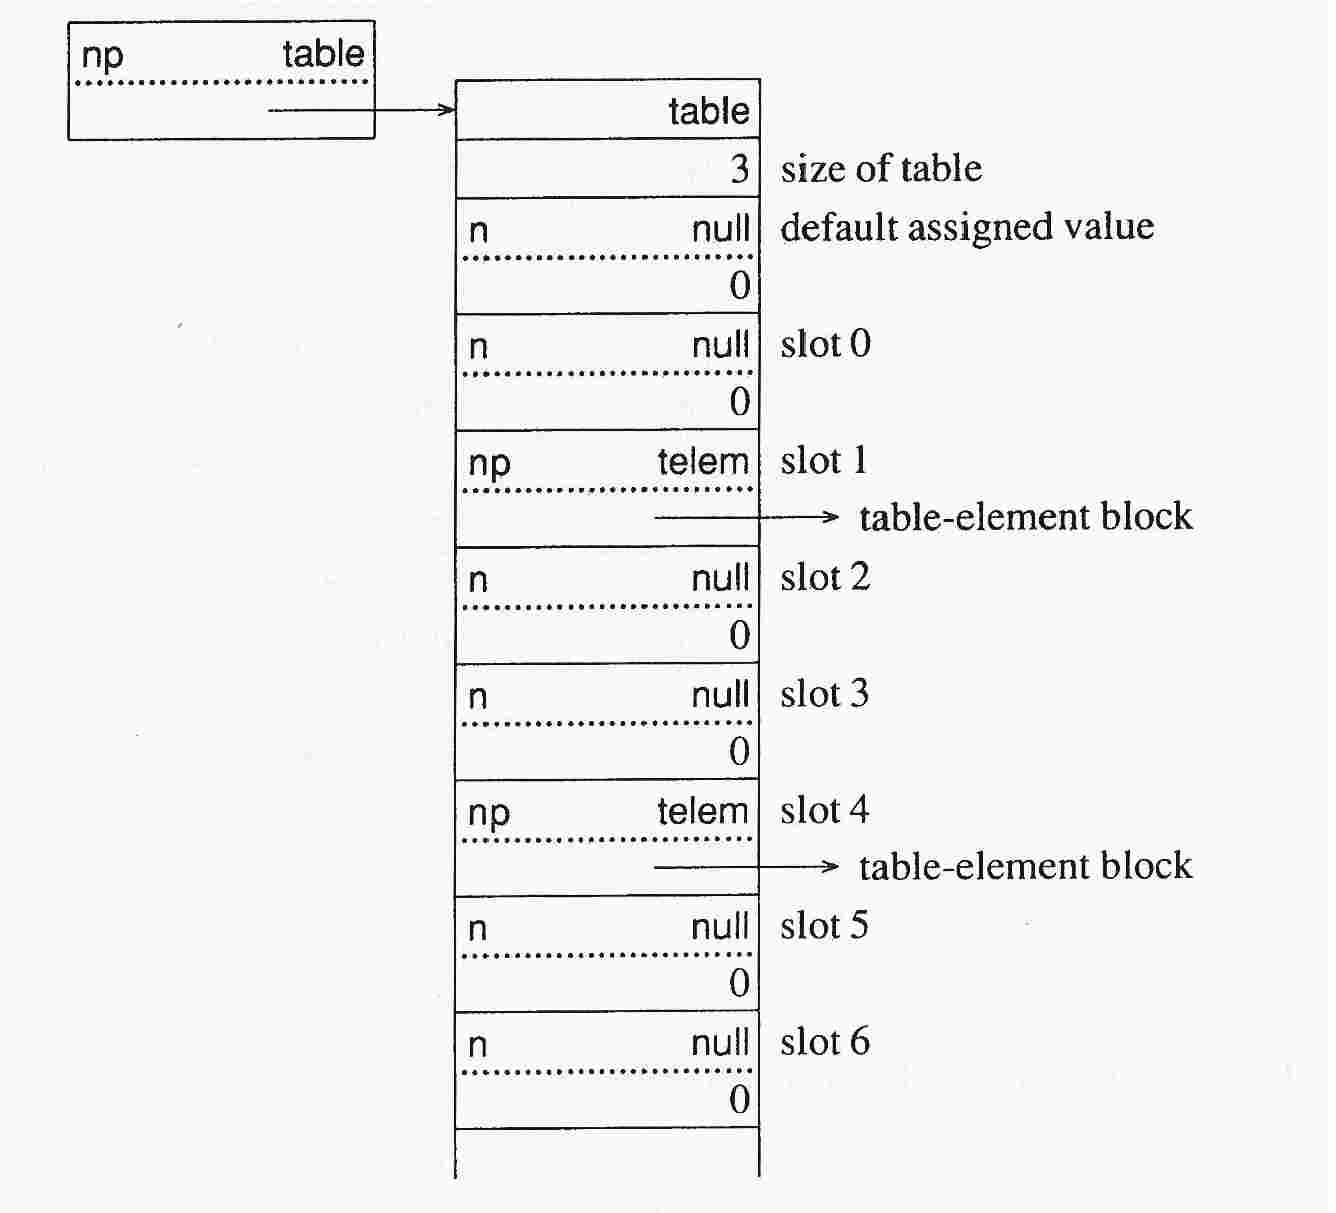
\includegraphics[width=4.489in,height=4.0516in]{ib-img/ib-img121.jpg} 


The table-element block for the entry value 4 in the previous example is


\ \  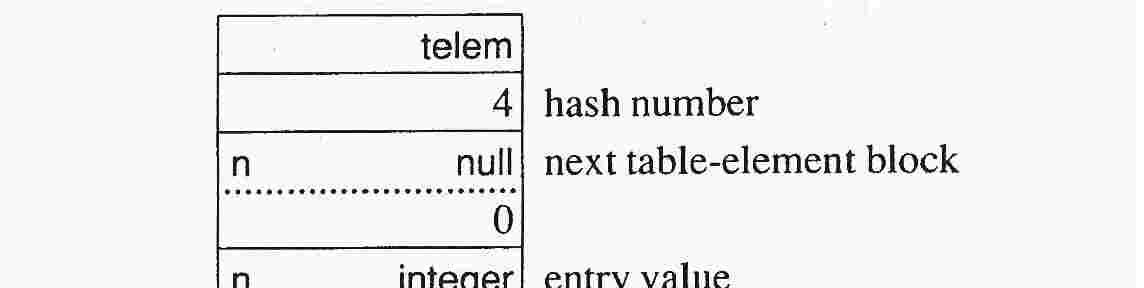
\includegraphics[width=3.848in,height=0.961in]{ib-img/ib-img122.jpg} 

\subsection[A.2.7 Procedures]{A.2.7 Procedures}

The procedure blocks for procedures and functions are similar. For a
procedure declaration such as

{\ttfamily\mdseries
\ \ procedure calc(i,j)}

{\ttfamily\mdseries
\ \ local k}

{\ttfamily\mdseries
\ \ static base, index}

{\ttfamily\mdseries
\ \ end}

\noindent the procedure block is


\ \  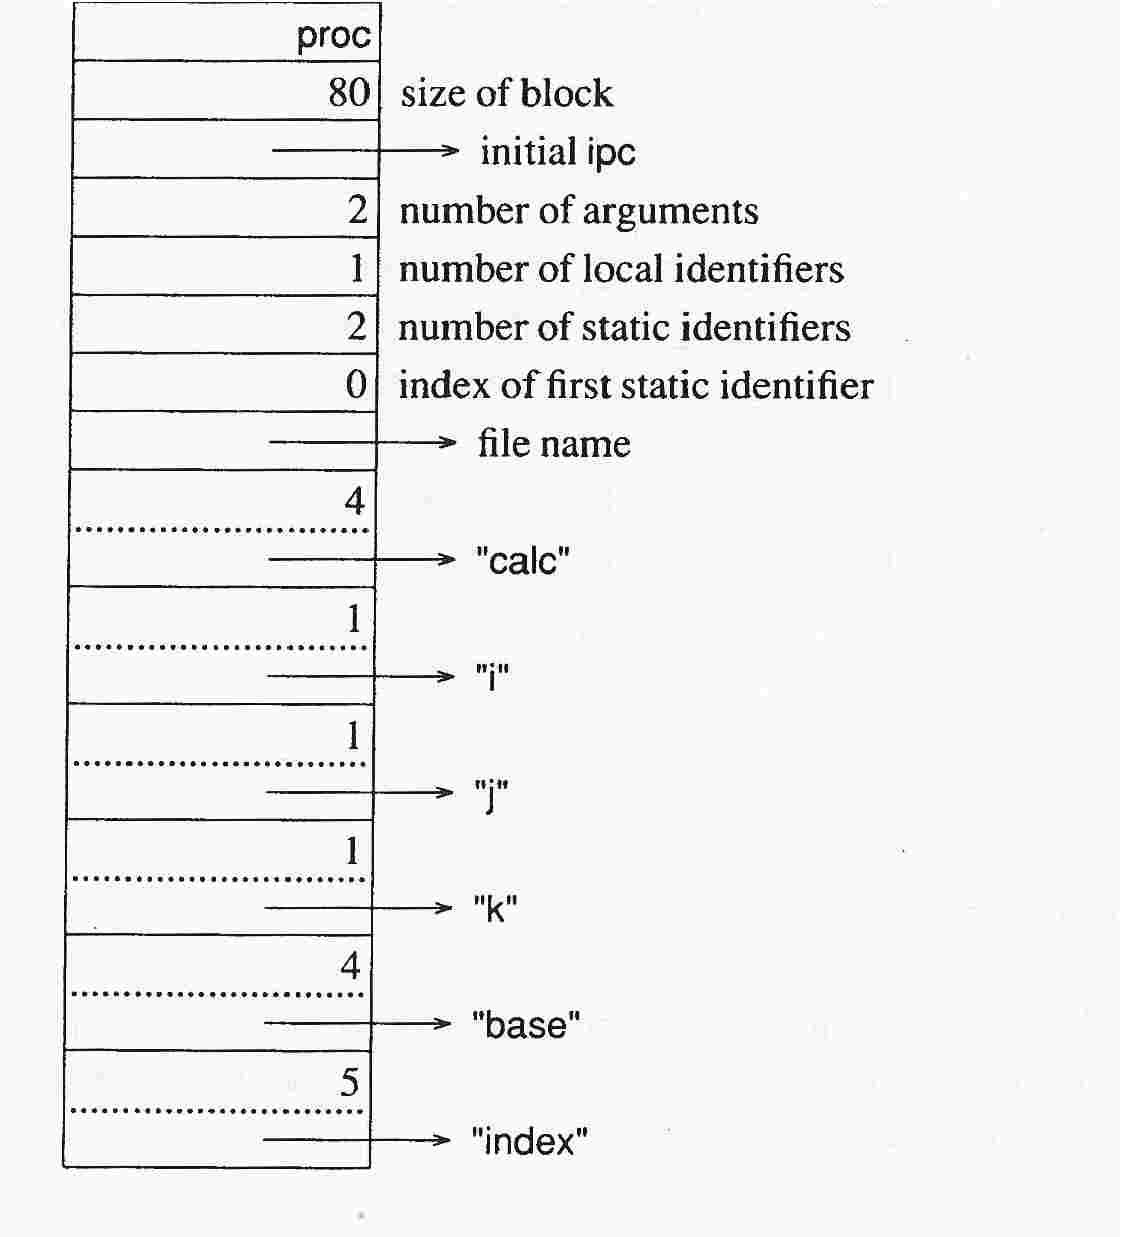
\includegraphics[width=3.848in,height=4.1307in]{ib-img/ib-img123.jpg} 


In a procedure block for a function, there is a value of -1 in place
of the number of dynamic locals. For example, the procedure block for
repl is


\ \  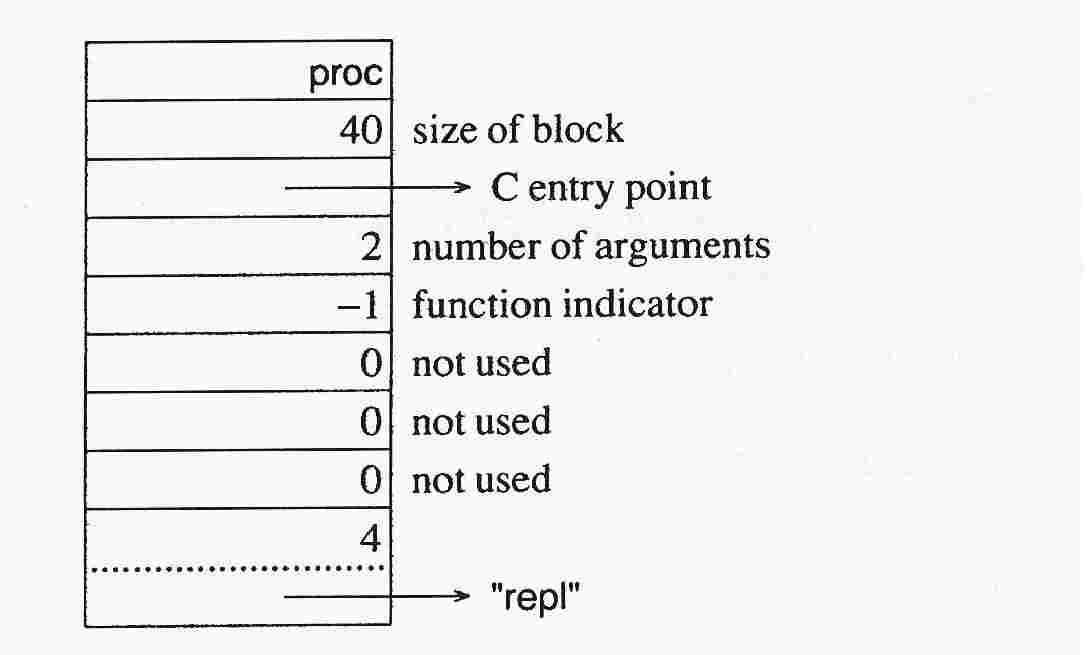
\includegraphics[width=3.6335in,height=2.1866in]{ib-img/ib-img124.jpg} 


In the case of a function, such as write, which has a variable number
of arguments, the number of arguments is given as -1:


\ \  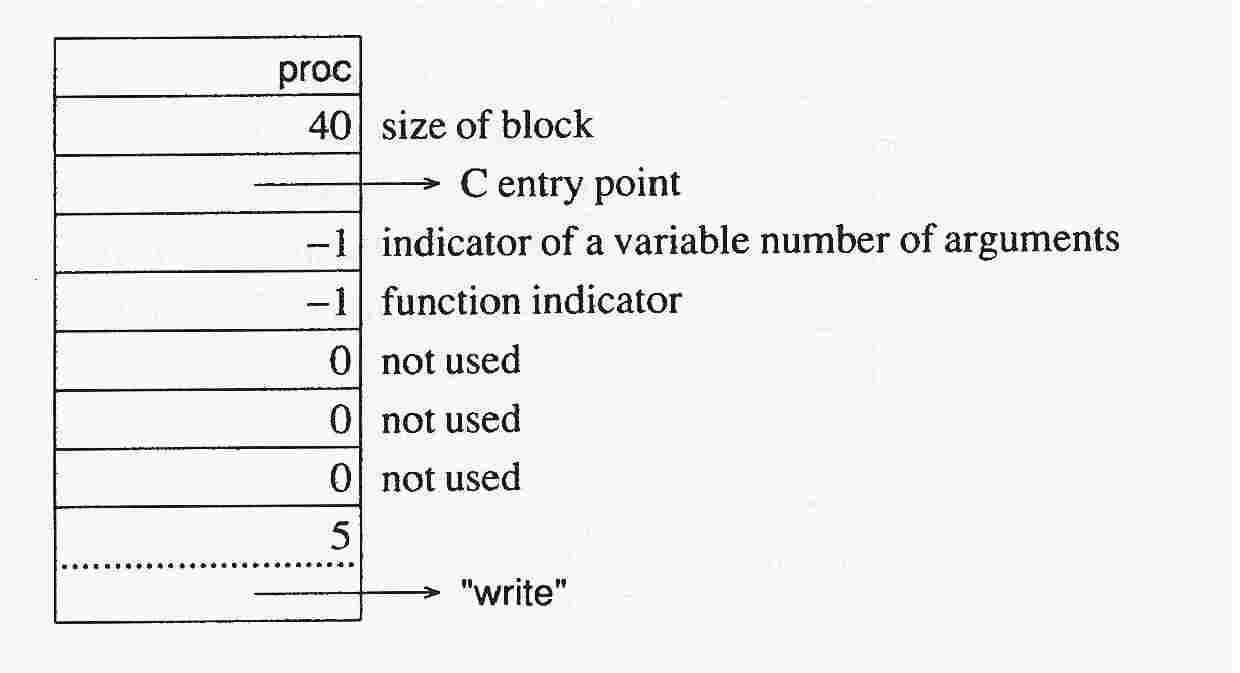
\includegraphics[width=4.1681in,height=2.248in]{ib-img/ib-img125.jpg} 

\subsection{A.2.8 Files}

The block for a file contains a pointer to the corresponding file, a
word containing the file status, and a qualifier for the name of the
file. For example, the block for \&output is


\ \  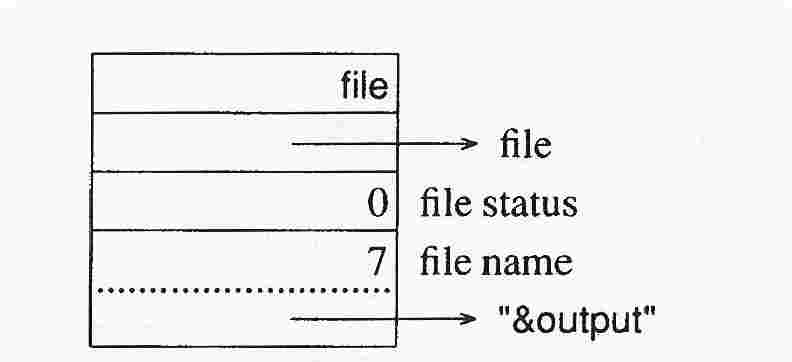
\includegraphics[width=2.6717in,height=1.2083in]{ib-img/ib-img126.jpg} 


The file status values are


\ \ 0 \ \ closed\newline
\ \ 1\ \ open for reading\newline
\ \ 2\ \ open for writing\newline
\ \ 4\ \ open to create\newline
\ \ 8\ \ open to append\newline
\ \ 16\ \ open as a pipe

\subsection{A.2.9 Trapped Variables}

There are three kinds of trapped variables: keyword trapped variables,
substring trapped variables, and table-element trapped variables. The
corresponding blocks are tailored to the kind of trapped variable.


The value of \&trace illustrates a typical keyword trapped variable:


\ \  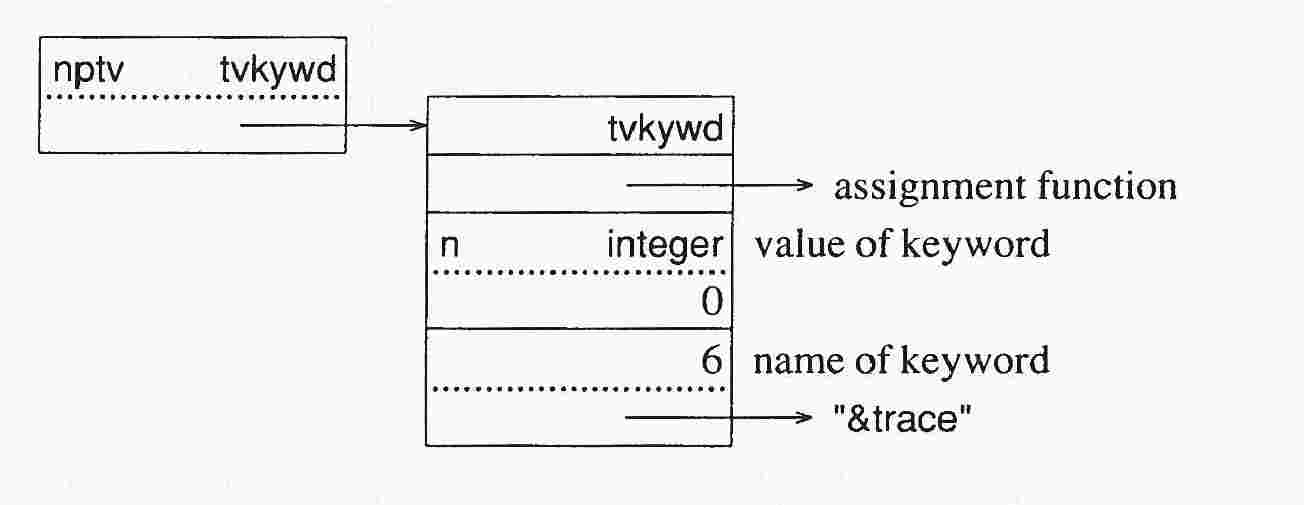
\includegraphics[width=4.3811in,height=1.6862in]{ib-img/ib-img127.jpg} 


A substring trapped variable contains the offset and length of the
substring, as well as a variable that points to the qpalifier for the
string. For example, if the value of s is
{\textquotedbl}abcdef{\textquotedbl}, the substring trapped-variable
block for s [2:5] is


\ \  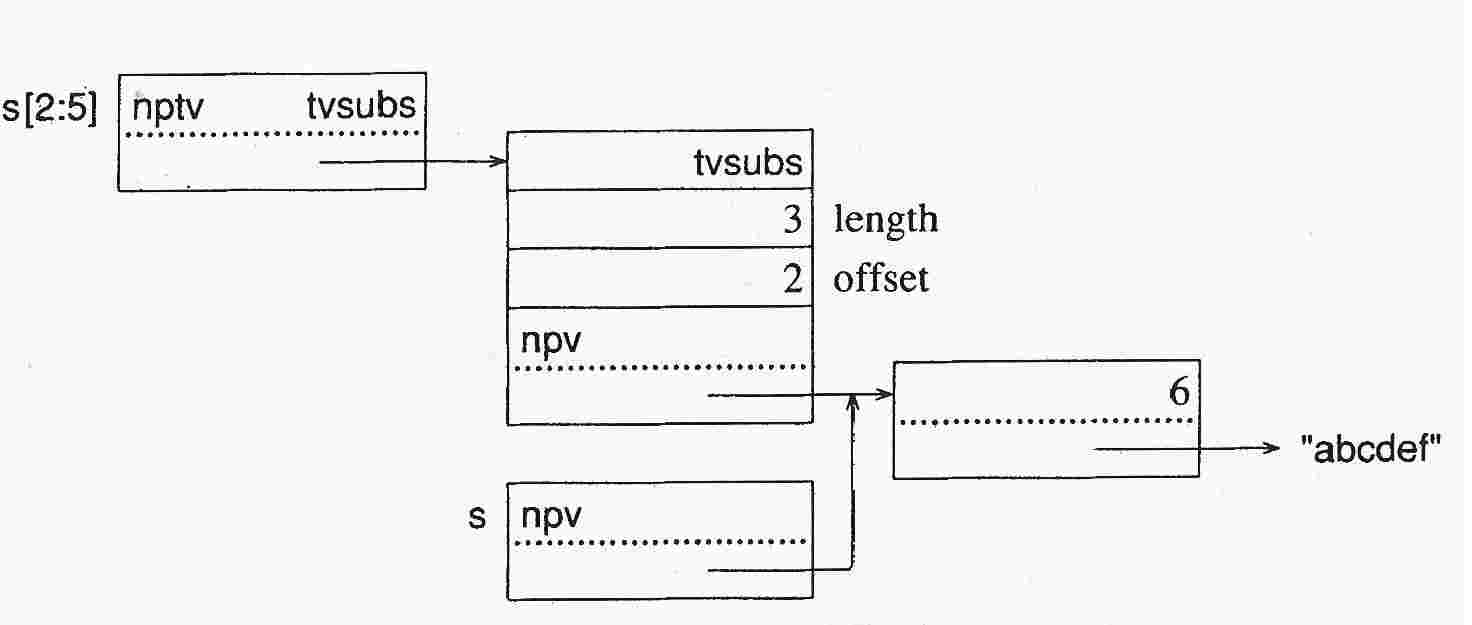
\includegraphics[width=4.9161in,height=2.0866in]{ib-img/ib-img128.jpg} 


A table-element trapped-variable block contains a word for the hash
number of the entry value, a pointer to the table, the entry value,
and a descriptor reserved for the assigned value. For example, if t is
a table, the table-element trapped-variable block for t[36] is


\ \  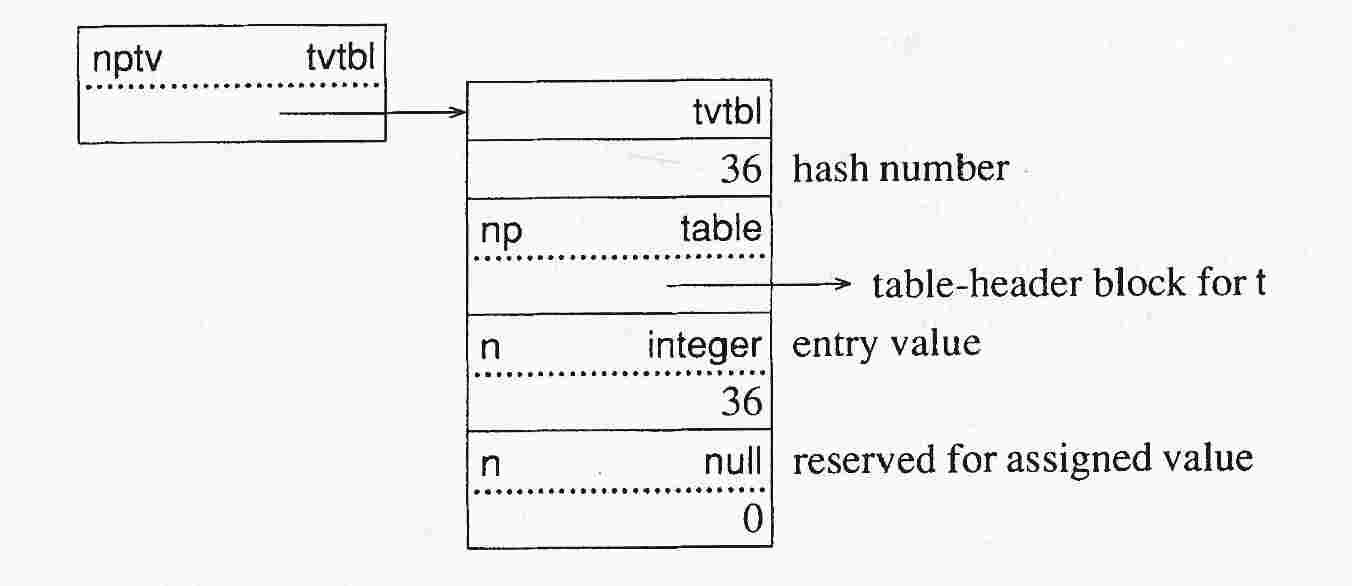
\includegraphics[width=4.5953in,height=1.9571in]{ib-img/ib-img129.jpg} 

\subsection{A.2.10 Co-Expressions}

A co-expression block consists of heading information, an array of
words for saving the C state, an interpreter stack, and a C stack:

\clearpage
\bigskip


\ \  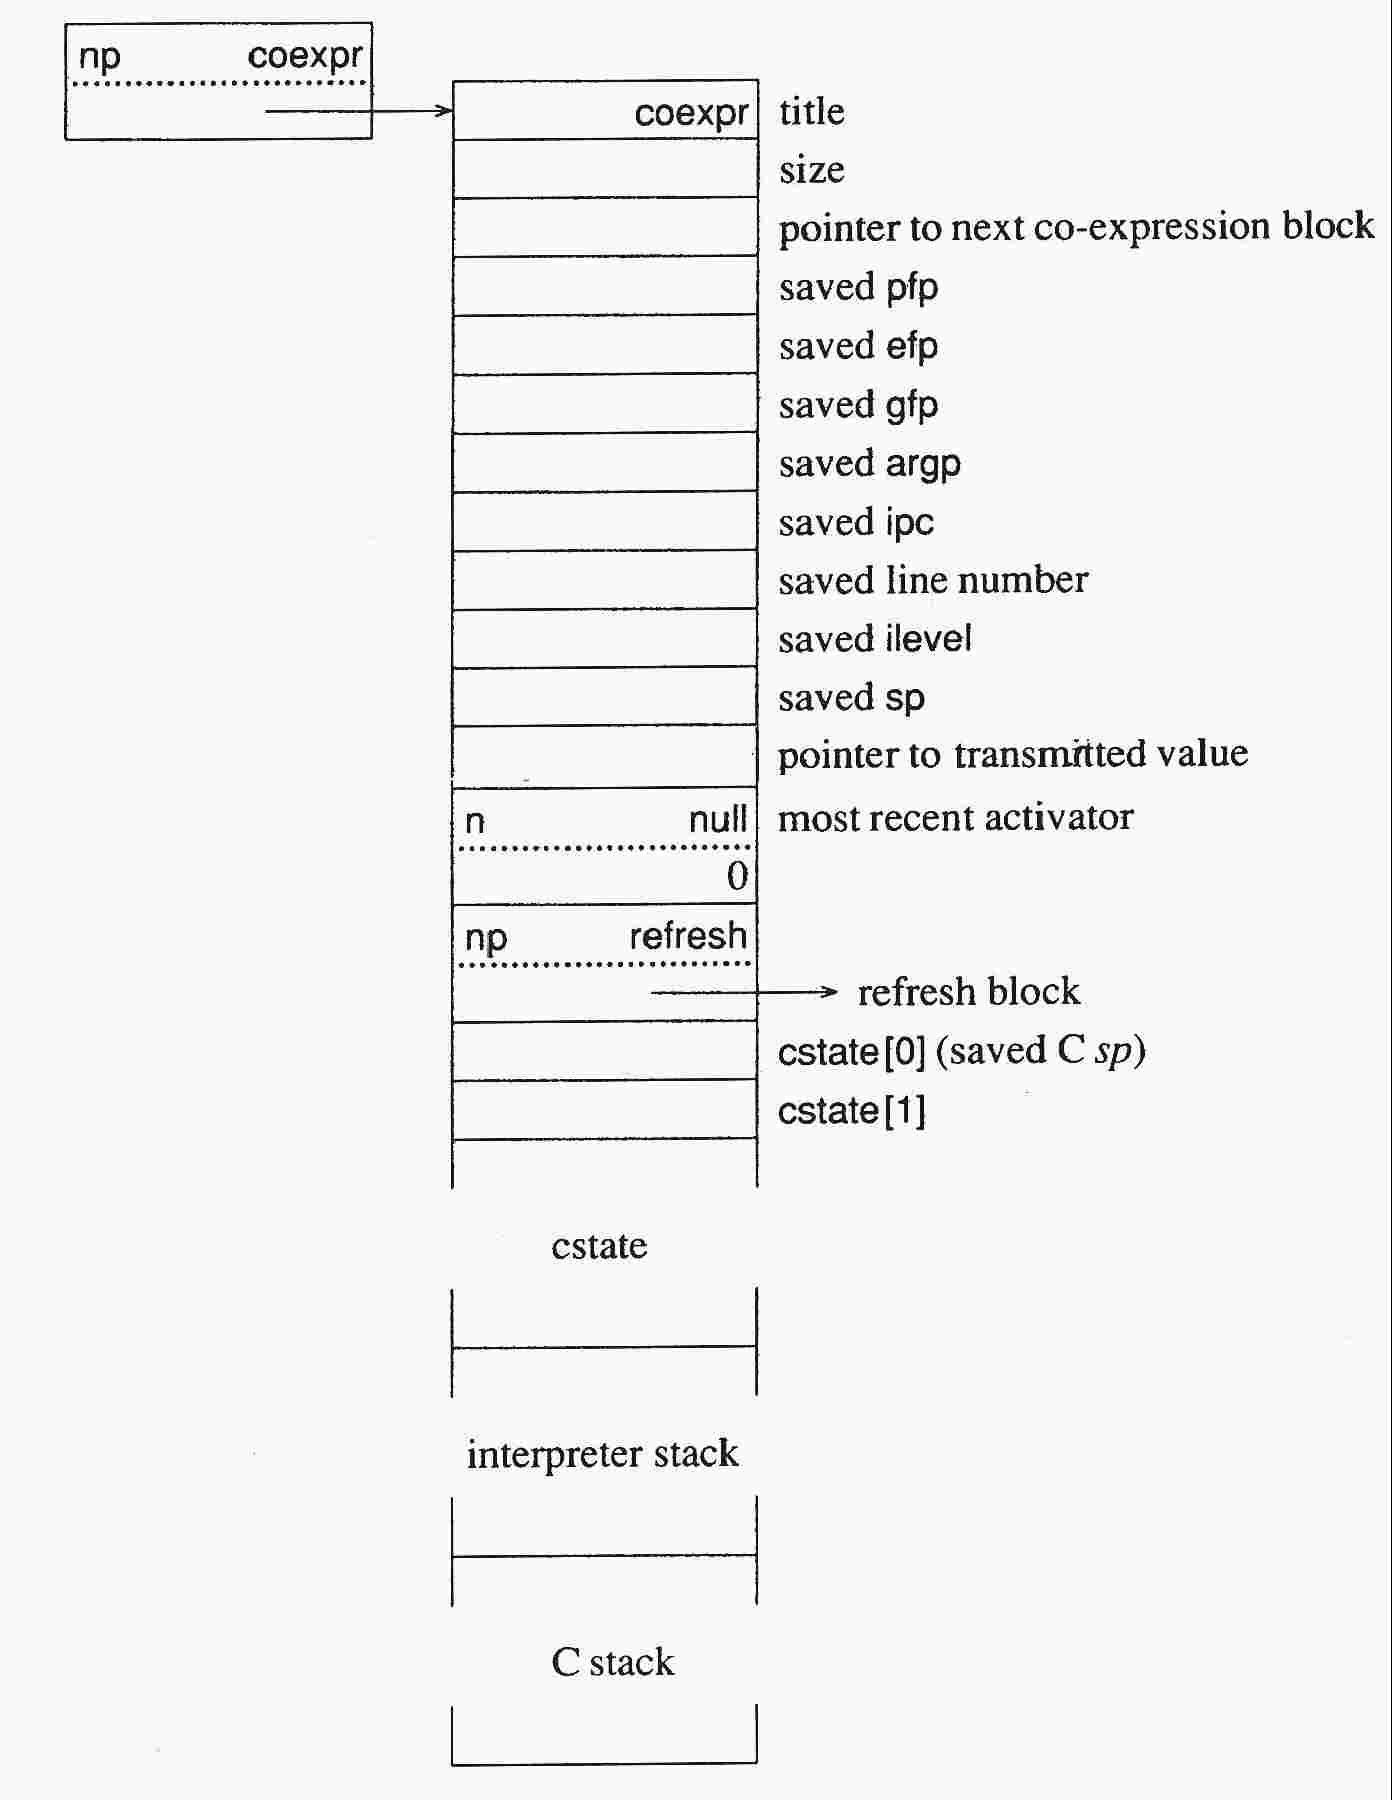
\includegraphics[width=4.702in,height=6.0126in]{ib-img/ib-img130.jpg} 


The refresh block contains information derived from the procedure
block for the procedure in which the co-expression was
created. Consider, for example,

{\ttfamily\mdseries
\ \ procedure labgen(s)}

{\ttfamily\mdseries
\ \ local i, j, e}

{\ttfamily\mdseries
\ \ i := 1}

{\ttfamily\mdseries
\ \ j := 100}

{\ttfamily\mdseries
\ \ e := create (s {\textbar}{\textbar} (i to j) {\textbar}{\textbar} {\textquotedbl}:{\textquotedbl})}

{\ttfamily\mdseries
\ \ ...}

{\ttfamily\mdseries
\ \ end}


For the call labgen({\textquotedbl}L{\textquotedbl}), the refresh block for e is


\bigskip


\bigskip


\bigskip


\bigskip


\bigskip


\bigskip


\ \  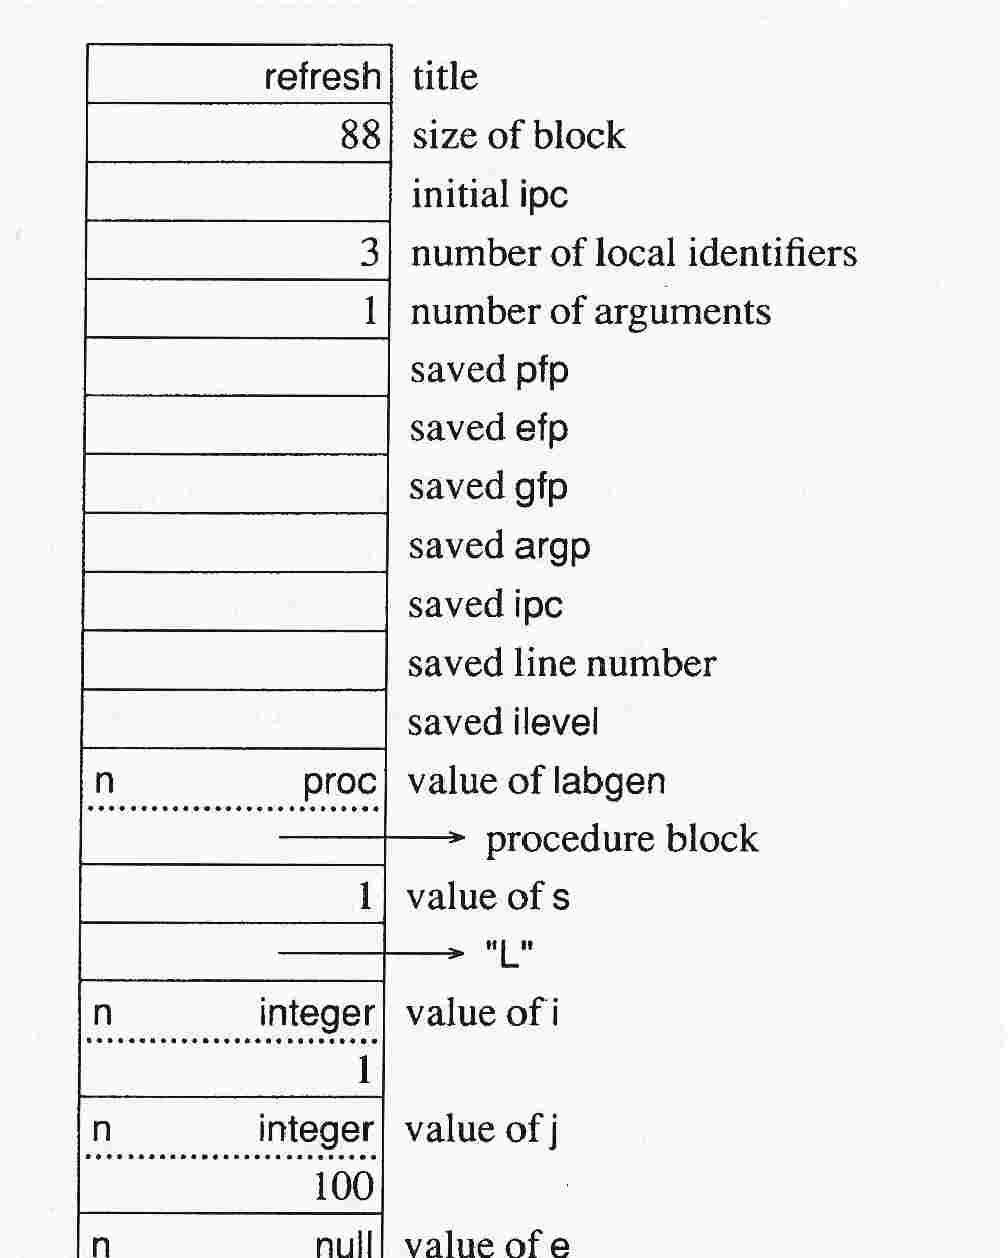
\includegraphics[width=3.4193in,height=4.2016in]{ib-img/ib-img131.jpg} 


\ \ \ \ \ \  \ \ 0
